\section{Scala macros}
Since we want to achieve compile time validation, we have to explicitly tell the Scala compiler. If the query would be defined as function, taking parameters, it would wait for runtime, when the parameters will be known (not just the types, as it is when compiling). And then each call to the function would be evaluated separately.

What we want to do is to validate query at compilation, so it creates at the parameter positions "placeholders". These will know the expected type, so every value passed to the function with matching type will result in valid query. In case the query is not valid, we will get compile time error right away, making it easier for us to debug the code and fix it.

That is where Scala macros are useful. They have same signature as functions, but their body consists of \texttt{macro} keyword and name of the macro function.  \textit{It will expand that application by invoking the corresponding macro implementation method, with the abstract-syntax trees of the argument expressions args as arguments.}~\cite{Def macros} I think that little description of what abstract syntax trees are is required here. In context of Scala, the AST is used as internal representation of the executed program. 

\subsection{Scala AST and Reflection library}
Macros are part of the Scala reflection library. We will specifically talk about the "Compile-time reflection". \textit{Scala reflection enables a form of metaprogramming which makes it possible for programs to modify themselves at compile time.}\cite{Compile-time reflection} 

When we enter execution of macro, we have the context and the function arguments. Everything is in the form of AST, so programming macros is slightly different from the usual programming in Scala. In simple terms context tells us where the macro was called from, which class, method name etc. 

\begin{figure}[h]
  \makebox[\textwidth]{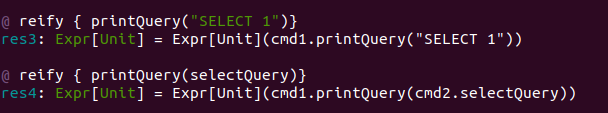
\includegraphics[width=\textwidth]{reify.png}}
  \caption {Differences in AST between parsing string directly and parsing variable}
\end{figure}

\subsection{Implementation}

\subsection{Lifting}

